\chapter{Background}\label{chap:background}

The explanations of the fundamental elements of reinforcement learning are based on the book Reinforcement Learning:
An Introduction\cite{Sutton1998} from Richard S. Sutton and Andrew G. Barto.

\section{Markov Decision Processes}
The Markov Decision Process (MPD)  is the mathematical framework of Reinforcement Learning and
is defined as a tuple < $\mathcal{S, A, R, T}$ >
\begin{itemize}
\item $\mathcal{S}$ is a set of states, s $\in \mathcal{R}^{n}$
\item $\mathcal{A}$ is a set of actions, a $ \in \mathcal{R}^{n}$
\item $\mathcal{R}$ is the reward
\item $\mathcal{T}$ is the transition probability function
\end{itemize}
Every state in a Markov Decision Process needs to satisfy the Markov Property,
which means that "The future is independent of the past given the present".
The definition is given by a state reward pair 
\begin{equation}
\mathcal{P}(S_{t+1}, R_{t+1} | S_{t}, R_{t}) =  \mathcal{P}(S_{t+1}, R_{t+1} | S_{t}, R_{t}, ..., S_{0}, R_{0})
\end{equation}
Unfortunately for most real-world problems this assumption is violated. This is also the case for the
state transition function, which is defined as
\begin{equation}
  \mathcal{P}(s_{t+1}| s_{t}, a_{t}) =  \mathcal{P}(S_{t+1} = s^{'}| S_{t} = s ,  A_{t} = a)
\end{equation}
 The goal of the agent is to find the policy that maximizes the total reward $(R_{t})$.
In the discounted case is given as 
\begin{equation}
  R_t = \sum^{\infty}_{k = 0} \gamma^k r_{t+k+1}
\end{equation}
with $\gamma$ as the discount factor to exponentially discounts future rewards. 
The policy is a function, which in the deterministic case maps states to actions.
While a stochastic policy $\pi(a|s)$ has a certain probability of selecting an action \textit{a} in state \textit{s}.
For every MDP there is always at least one optimal policy $\pi$. 
In case the transition probability is given, the \textit{dynamic programming} based \textit{value iteration} Algorithm is one way to compute policy $\pi$.
This Algorithm is build upon the concept of a value function.
\subsection{Value Function}
The value function $V^{\pi}$ : $\mathcal{S}$ $\rightarrow$ $\mathcal{R}$, represents the expeceted total reward in a given state when following the policy $\pi$.
It is defined as
 \begin{equation}
  \begin{aligned}
    V^{\pi}(s) &= \mathbb{E}_{\pi} [R_t | s_t = s] \\
    &= \mathbb{E}_{\pi} [\sum^{\infty}_{k=0} \gamma^{k} r_{t+k+1} | s_t = s] \label{MDP:eq1} \\
    &= \sum_{a \in \mathcal{A}} \pi(s, a) \sum_{s' \in \mathcal{S}} \mathcal{T}^{a}_{ss'}[\mathcal{R}^{a}_{ss'} + \gamma V^\pi(s')]
  \end{aligned}
\end{equation}
In each Iteration \textit{i} of the \textit{value iteration} Algorithm the value function is updated by the following equation
\begin{equation}
  V_{i+1}(s) := \max_a \Big\{ \sum_{s', r} P(s',r| s,a) (r + \gamma V_i(s')) \Big\}
\end{equation}
This update is repeated until both sides of the equation are equal.
\subsection{Q-value Function}
In many real-world problems the transition function is unknown and computing the value function is not feasible, because
it would require evaluating all possible actions in a single state at every time step.
To evaluate every action in a state the Q-value function $ \mathcal{Q}: \mathcal{S} \times \mathcal{A} \rightarrow \mathcal{R} $
\begin{align}
  Q^{\pi}(s, a) &= \textsc{E}_\pi[R_t | s_t = s, a_t = a] \\
  &= \textsc{E}_\pi [\sum^\infty_{k=0} \gamma^k r_{t+k+1} | s_t = s, a_t = a]
\end{align}
It represents the expected reward of the agent if the action a is chosen in state s at time step t when following the current policy $\pi$.
The Bellman Optimality Equation is one way to update the Q-value Function 
\begin{equation}
  Q(s_t, a_t) \leftarrow Q(s_t, a_t) + \alpha[r_{t+1} + \gamma \max_a Q(s_{t+1}, a) - Q(s_t, a_t)]
\end{equation}
where $ \alpha$ is the \textit{learning rate} and $\gamma$ weights between short and longterm reward.

\subsection{Q Learning}
This update equation is used to find an optimal policy in the Q-Learning Algorithm repesened in Algorithm \ref{alg:q-learning}
\begin{algorithm}[H]
\caption{Q-learning}
\label{alg:q-learning}
\begin{algorithmic}
    \State Algorithm parameters: learning rate $\alpha \in (0, 1]$, discount factor $\gamma \in (0, 1]$, exploration rate $\epsilon > 0$
    \State Initialize $Q(s,a)$ randomly except $Q(terminal, \cdot) = 0$
    \While{not converges}
        \State Set initial state $s$  
        \While{$s$ is not terminal}
            \State With probability $\epsilon$:
            \State \hspace{\algorithmicindent} Pick random action $a$
            \State otherwise:
            \State \hspace{\algorithmicindent} $a$ = argmax$_a$ $Q(s, a)$
            \State Execute action $a$ and observe reward $r$ and succesor state $s'$
            \State$Q(s, a) \leftarrow Q(s, a) + \alpha[r + \gamma \max_{a^*} Q(s', a^*) - Q(s, a)]$
            \State $s \leftarrow s'$
        \EndWhile
    \EndWhile
\end{algorithmic}
\end{algorithm}

The Algorithm is based on the concept of Temporal Difference Learning.
It uses the combined ideas of Dynamic Programming (DP) and Monte Carlo (MC) methods.
Like in Dynamic Programming the old estimate to update the new estimate. Unlike MC it uses a bootstraped estimate.

Q-Learning is an off-policy Algorithm, it uses different policies for interacting with the environment and updating the Q-value Function.

\section{Neural Network}
In complex environments, the state space is continuous, which makes it infeasible to store all state-action pairs in a table.
Advances in machine learning especially in deep learning make it possible to approximate the Q function.  
Basic elements of Deep learning are artificial neural networks which are inspired by the human brain.
Neural network have a structure of input layer connected to hidden layers followed by the output layer. 
A fully connected network has many hidden layers represented as nodes. The nodes between different layers are connected by weights. 
The values of the weights can be trained iteratively by using an optimization technique like stochastic gradient descent and backpropagation.
This simple architecture could be seen as matrix multiplications which makes it a linear function.
By adding nonlinear activation functions it is able to approximate more complex nonlinear functions.
\begin{figure}[h]
  \centering
  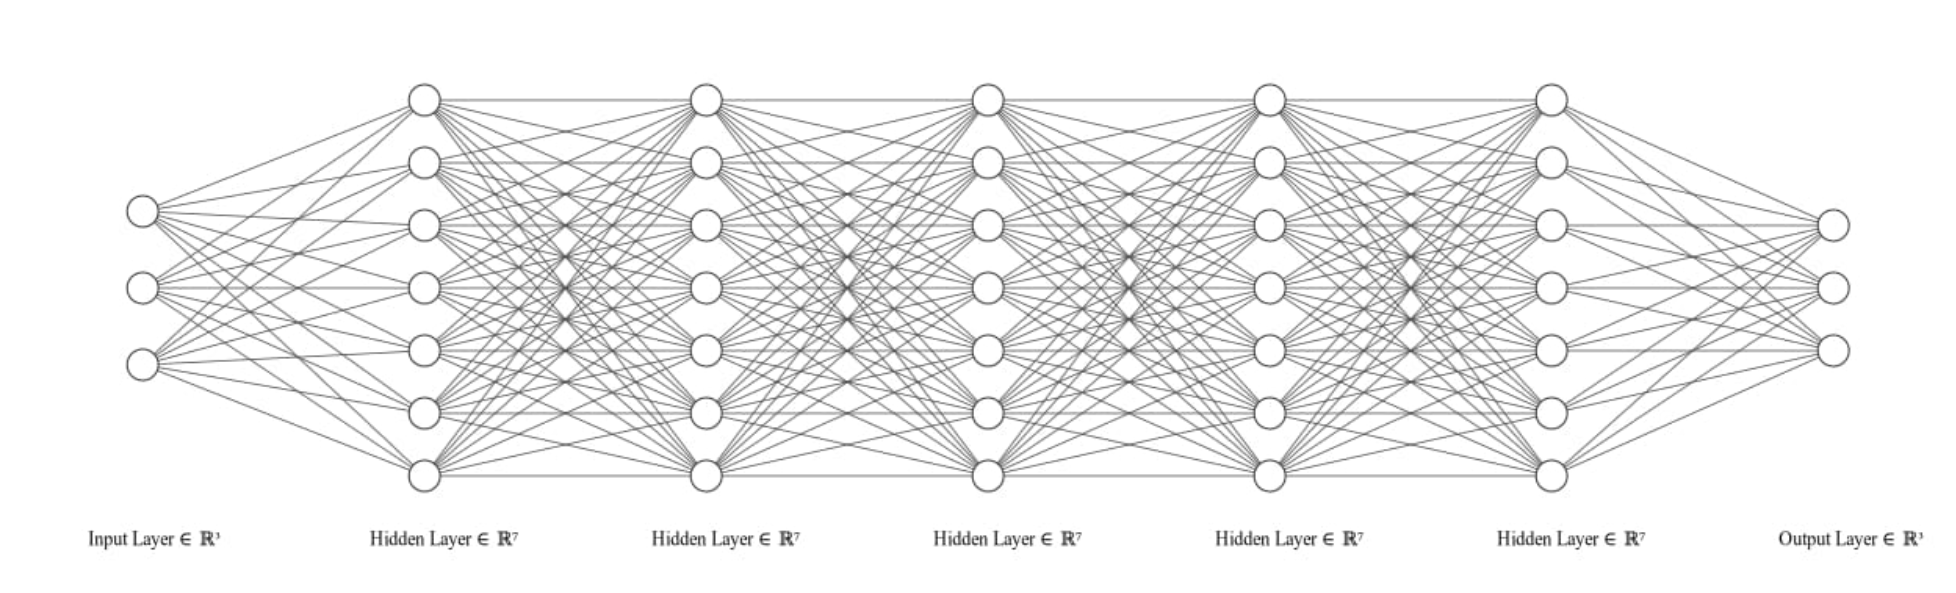
\includegraphics[width=0.5\textwidth]{figures/background/nn.png}
  \caption{Deep Neural Network with several hidden layers}
  \label{fig:tab-training}
\end{figure}



\section{Soft Q Learning}

Soft Q learning uses the maximum entropy to augment the standard RL objective 
by maximizing also the entropy of the policy. 

\begin{equation}
  \pi^* = \underset{\pi}{\mathrm{argmax}} \sum_{t=0}^{T} E_{(s_t, a_t) \sim \tau_{\pi}}[\gamma^t (r(s_t, a_t) + \alpha \mathcal{H}(\pi(.|s_t))]
\end{equation}

The entropy of the polciy $\pi$ is represented by $\mathcal{H}(\pi(.|s_t))]$ and is computed with $-log\pi(.|s_t)$.
This new objectiv leads to a stochasic policy and an implicit exploration.
In most cases it is difficult to find a good $\alpha$, for this nt. Haarnoja et al. (2018) proposed to adjust $\alpha$  dynamically by taking a
gradient step with respect to the loss 

\begin{equation}\label{eq:entropy_temp}
J(\alpha)= \mathbb{E}_{\mathcal{D}, \pi}
\left[
    \log \alpha \cdot  (
        -\log \pi( a_{t} | s_{t} )
        -
        \mathcal{H}_T
    )
\right],
\end{equation}


\section{Actor-Critic Concept}

The Algoritem used in this work is based on Soft Q Learning approch and the Actor-Critic Concept.

The Actor is a Neural Network to approximate our policy function p(s) in continuous action spaces.  
This is necessary because with infinite actions the max operation for updating the Q-value function is not feasible. The probably simplest way to update the 
actor weights to force the actor to select actions that have a higher Q-value is by using the critic to evaluate the actions.

A simple way is to minimize the policy gradient loss:

\begin{equation}
  \nabla_{\theta} \mathcal{L}_{\theta}(\mathcal{D}) = - \mathbb{E}_{s \sim \mathcal{D}} [\nabla_{\theta} log \pi_{\theta}(a|s) \cdot Q_{\phi}(s,a)]
\end{equation}


The Critic is used to evaluate the action of the actor. It is a neural network that approximates the Q-value function and it can be trained by minimixing the mean squard error loss
of the training data-set $\mathcal{D}$ represented by the replay buffer. 

\begin{equation}
  \mathcal{L}_{\phi}(\mathcal{D}) =  \mathbb{E}_{s,a, r, s^{\prime} \sim \mathcal{D}} [Q_{\phi}(s,a) - \underbrace{( r + \gamma \: \underset{a^{\prime}}{max} \:  Q_{\phi^{\prime}}(s^{\prime},a^{\prime})}_{TD - target}]^{2}
\end{equation}



